% !TEX root = main.tex  

\section{\href{https://www.youtube.com/watch?v=hS47TcdiKUU}{Beggining and struggles in the age of genomics}.}

\paragraph{Notes about the video:}

\paragraph{\\}
\begin{figure}[htbp]
    \centerline{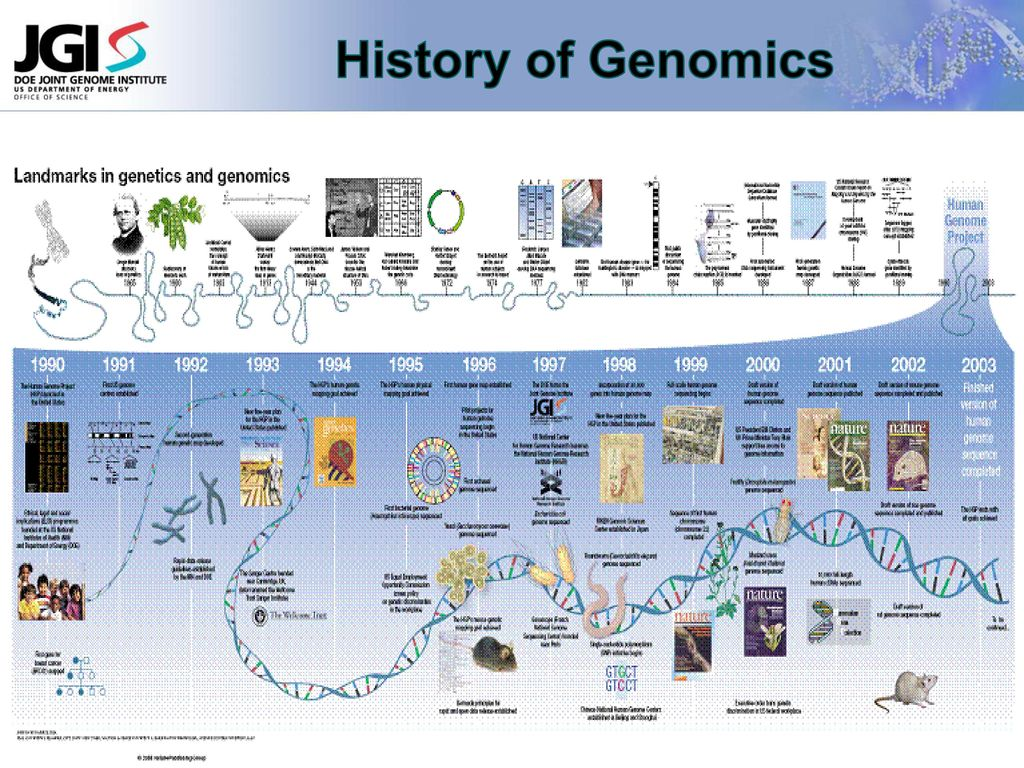
\includegraphics[width=200mm]{historyGenomics.jpg}}
    \caption{History of Genetics}
    \label{fig4}
\end{figure}

\section{Important years}
1865: Laws of genetics (Mendel laws). \\
1900: Darwin theory + Mendel laws join together \\
1913: Alfred Henry first linear genetic maps \\
1953: Watson and Crick discover the structure of DNA \\
1966: Determination of the genetic code \\
1977: Creating of the first methods to sequence DNA \\
1982: GenBank database was established \\ 
1985: Discovery of the chain reaction polymerase \\
1988: They start to talk about the human genome project \\
1990: The human genome starts and the ELS(Ethical, legal and social implications) \\
1993: The wellcome Trust Sanger Institute \\
1997: Joint Genome institue and National Humans Genome Research Institute (JGI and NHGRI)\\
2003: Finished version of the human genome sequence completed \\

\paragraph{Challenges}
Biology: Concrete the structure and function of the genomes. \\
Health: Find benefits based on the human genome knowledge. \\
Society: Use genomics to maximize the benefis and minimize dangers in society. \\


\begin{itemize}
    \item Humans share 99 of their DNA.
    \item Thymine gets along with Adenine. (hydrogen bonding)
    \item Guanine gets along with Cytosine. (hydrogen bonding)
    \item Model organisms: yeast, bacteria.
\end{itemize}

\paragraph{The three biggest challenges: }

\begin{itemize}
    \item Indentify the functional and structural components in the HG.
    \item Understand the organization of the genetic networks and protein routes to see how
    they corelate to the phenotype in organisms.
    \item To develop a detailed hereditary variation in the HG.
    \item To comprehend biggest
\end{itemize}
